\documentclass[conference]{IEEEtran}
\ifCLASSINFOpdf

\newcommand{\redcolor}[1]{\textcolor{red}{#1}}

\newcommand{\figref}[1]{Figure~\ref{#1}}
\newcommand{\secref}[1]{Section~\ref{#1}}
\newcommand{\tabref}[1]{Table~\ref{#1}}
\newcommand{\algoref}[1]{Algorithm~\ref{#1}}
\usepackage{graphicx}
\usepackage{subfig}
\usepackage{blindtext}
\usepackage{array}
\usepackage{caption}
\usepackage{url}
\usepackage{epstopdf}
\usepackage{multirow}

%\usepackage[pdftex]{graphicx}
% % declare the path(s) where your graphic files are
%\graphicspath{{../figures/}}
%  % and their extensions so you won't have to specify these with
%  % every instance of \includegraphics
%\DeclareGraphicsExtensions{.pdf,.jpeg,.png}
\else
\fi
% *** MATH PACKAGES ***
%
%\usepackage[cmex10]{amsmath}
% *** SPECIALIZED LIST PACKAGES ***
\usepackage[linesnumbered,ruled,vlined]{algorithm2e}

% *** ALIGNMENT PACKAGES ***
%
%\usepackage{array}
%\usepackage{mdwmath}
%\usepackage{mdwtab}
%\usepackage{eqparbox}
% *** SUBFIGURE PACKAGES ***
%\usepackage[tight,footnotesize]{subfigure}
%\usepackage[caption=false]{caption}
%\usepackage[font=footnotesize]{subfig}

% *** FLOAT PACKAGES ***
%
%\usepackage{fixltx2e}
%\usepackage{stfloats}
% *** PDF, URL AND HYPERLINK PACKAGES ***
%\usepackage{url}
% correct bad hyphenation here
\hyphenation{op-tical net-works semi-conduc-tor}


\begin{document}
%
% paper title
% can use linebreaks \\ within to get better formatting as desired
\title{INDiC: Improved Non intrusive load monitoring using load Division and Calibration}


% author names and affiliations
% use a multiple column layout for up to three different
% affiliations
\author{\IEEEauthorblockN{Author1}
\IEEEauthorblockA{Indraprastha Institute of Information Technology\\
India\\
}
\and
\IEEEauthorblockN{Author2}
\IEEEauthorblockA{Twentieth Century Fox\\
Springfield, USA\\
Email: homer@thesimpsons.com}
\and
\IEEEauthorblockN{James Kirk\\ and Montgomery Scott}
\IEEEauthorblockA{Starfleet Academy\\
San Francisco, California 96678-2391\\
Telephone: (800) 555--1212\\
Fax: (888) 555--1212}}
% make the title area
\maketitle


\begin{abstract}
%\boldmath
Non-Intrusive appliance load monitoring (NIALM) is the process of disaggregating the overall electricity usage into constituent appliances. In this paper we extend the Combinatorial Optimization (CO) approach for disaggregation, which was originally proposed in the seminal work on NIALM, in following two ways: 1) Breaking the problem into subproblems and reducing the state space; 2) Applying additional constraints backed by sound domain expertise. We evaluate our approach using REDD dataset and show practical problems which need to be solved while dealing with the dataset. We also propose a metric for evaluating NILM, which we believe overcomes many shortcomings of commonly used metrics.
\end{abstract}
\IEEEpeerreviewmaketitle



\section{Introduction}
% no \IEEEPARstart
\begin{itemize}
\item Motivate the importance of energy consumption in building
\item Motivate that appliance level information is crucial - detailed feedback and optimized decision making \cite{darby}
\item Challenges with getting appliance level information - introduce NIALM~\cite{hart}
\item introduce your proposed approach
\item Enumerate the contributions
\end{itemize}

Primary contributions of our work are:
\begin{itemize}
\item Fill it up with 2-3 crisp points
\end{itemize}
Open source implementation of the proposed work is released for comparative analysis with other NIALM approaches as an IPython notebook\footnote{\url{http://www.ipython.org}}. We believe this is the first extensive release of a generic NIALM

\section{Related work}
NIALM has been well studied in the recent past and survey papers \cite{survey1,survey2,survey3} present its classification across various dimensions. Following are three important classification dimensions:
\begin{itemize}
\item \textbf{Frequency of data collection}: Approaches such as harmonic analysis require data to be sampled at more than a thousand samples a second. Whereas approaches 
\item \textbf{Supervised/Unsupervised}: 
\end{itemize}
When you do the comparison, bring up how is your work different rather than just saying X did A and Y did B.
\begin{itemize}
\item Classification of different NIALM approaches - High/Low frequency, Time/Frequency domain analysis, supervised/unsupervised~\cite{survey1,survey2,survey3}.

For a more detailed overview the reader is referred to the above mentioned survey papers.

\item Discuss the modeling approaches that are used
\begin{itemize}
\item Additive Factorial HMM
\item Difference HMM \cite{parson2012_aaai}
\end{itemize}

\item Datasets used: Recent datasets have spurred this field
\begin{itemize}
\item REDD \cite{redd}
\item Blued \cite{blued_cmu}
\item Smart* \cite{smart}
\end{itemize}

\end{itemize}


\section{NIALM}
NIALM is the process of disaggregating the total electrical load into constituent appliances \cite{hart}. A typical NIALM setup involves instrumenting the power mains with smart meters and the aim is to attribute the whole home electricity load perceived at the smart meter into different appliances. \figref{fig:disagg} shows the house mains disaggregated into 3 appliances.

\begin{figure} 
	
    \subfloat[\scriptsize Aggregate Power]{
    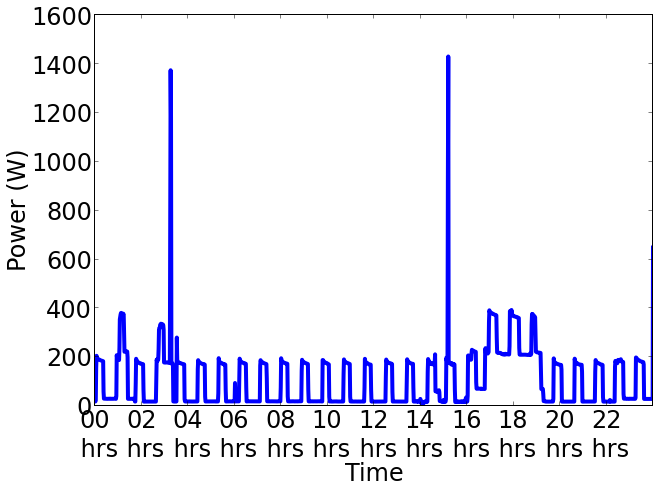
\includegraphics[scale=0.20]{./figures/before_disagg.png}}
    \subfloat[\scriptsize Disaggregated Power]{
        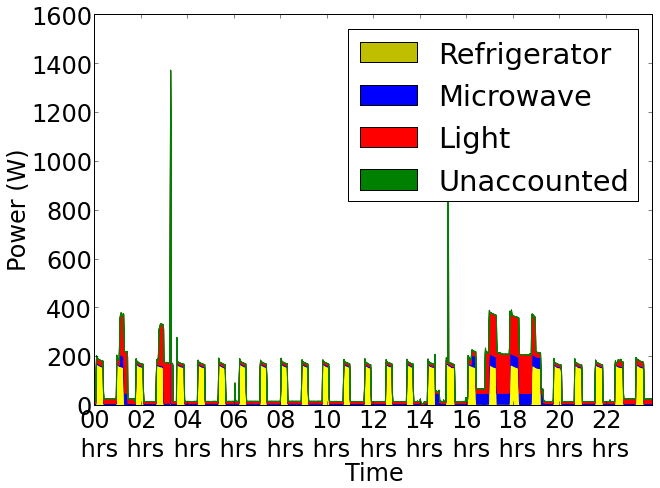
\includegraphics[scale=0.20]{./figures/after_disagg.png}}
  	\caption{The process of disaggregation}
    \label{fig:disagg}
\end{figure}
We use some terminologies from previous work and introduce some which are needed for our analysis in \tabref{tab:terms}. Based on these terminologies the NIALM problem in supervised setting may be formulated as predicting the power sequence for $n^{th}$ appliance, given by $y^n$, given the labeled power sequence for each appliance $\theta^n$ and the total aggregate power sequence $x$.


\begin{table}
\caption{Terminologies and Functions}
\label{tab:terms}
\begin{tabular}{|l|l|}
\hline
Symbol&Meaning\\
\hline
$t\in {1,..T}$& Time slice\\
$n\in{1,..N}$ & Appliance number\\
$\theta^n=\{\theta_1^n,...,\theta_T^n\}$ & Labeled power sequence for each appliance\\
$\theta^{M_1}=\{\theta_1^{M_1},...,\theta_T^{M_1}\}$ & Labeled power sequence for Mains 1\\
$\theta^{M_2}=\{\theta_1^{M_2},...,\theta_T^{M_2}\}$ & Labeled power sequence for Mains 2\\
$x=\{ x_1,..,x_T\}=\theta^{M_1}+\theta^{M_2}$ & Labeled aggregate power sequence\\
$v=\{ v_1,..,v_T\}$ & Labeled voltage time series\\
$e^{M_1}=\{e_1^{M_1},...,e_T^{M_1}\}$ & Noise power sequence for Mains 1\\
$e^{M_2}=\{e_1^{M_2},...,e_T^{M_2}\}$ & Noise power sequence for Mains 2\\
$e=\{e_1,...,e_T\}$ & Aggregate noise power sequence\\
$y^n=\{y_1^n,..y_T^n\}$ & Predicted power sequence for $n^{th}$ appliance\\
$k\in {1,..K}$ & Appliance power state\\
$z^n=\{z_1^n,..z_T^n\}$ & Appliance state sequence,$z_i^n \in [1,..K]$\\
$z_{t,k}^n \in{0,1}$ & 1 of K coding for whether $n^{th}$ \\
&appliance is in $k^{th}$ state at time $t$\\
$\mu^n=\{\mu_1^n,..\mu_K^n\}$ & Power draw by $n^{th}$ appliance in $k^{th}$ state\\
$Mapping[n] \in {1,2}$ & Mapping of $n^{th}$ appliance to Mains\\
\hline
\multirow{2}{*}{$B$} & List of background appliances (which can run\\
 					 &without human intervention) eg. refrigerator\\
\multirow{2}{*}{$F$} & List of foreground appliances (which are \\ 
 					 &operated by humans) eg. light, microwave\\
\hline
$Downsample(s,filter,$ & Function to downsample a timeseries $s$ to\\
$interval)$                                        & an $interval$ according to specified $filter$\\
\multirow{2}{*}{$Align([s^1,..s^n],method)$} & Function to align $n$ timeseries accounting\\
                                        &for missing data using specified $method$\\
\multirow{2}{*}{$Sort([s^1,..s^n],rule,order)$} & Function to sort $n$ timeseries according\\
                                        &to $rule$ in specified $order$\\
$Contiguous\_Below\_$ & Function to find contiguous period where time \\
$Mean(s,min\_period)$                  &series $s$ is below its mean \\
                                       &for atleast $min\_period$\\
$Step\_Changes(s,$ & Function returning magnitude and times of step\\
$threshold,interval)$                  &changes occurring in time series $s$ during \\
                              &an $interval$ , whose absolute value is \\
                              & greater than $threshold$\\
\multirow{2}{*}{$Greater\_Than(s,threshold)$} & Function to return times when timeseries $s$ is\\
                                        &greater than $threshold$\\                                                                                                    
                                                                               

\hline
%
\end{tabular}
\end{table}

\textbf{Combinatorial optimization}:
We follow 1-of-K coding scheme for appliance states and thus we have:
\begin{equation}
\sum\limits_{k=1}^{k=K} z_{t,k}^n=1
\end{equation}
The power consumption by $n^{th}$ appliance in $k^{th}$ state at time $t$ is given by:
\begin{equation}
\hat{\theta}^n_{t,k}=\sum\limits_{k=1}^{K} z_{t,k}^n \mu_k^n
\end{equation}
The overall power consumption of all appliances at a given time $t$ is given by:
\begin{equation}
\hat{x}_{t}=\sum\limits_{n=1}^{N}\sum\limits_{k=1}^{K} z_{t,k}^n \mu_k^n
\end{equation}
The error in power signal after the load assignment explained above is given by:
\begin{equation}
e^t=|x_t-\sum\limits_{n=1}^{N}\sum\limits_{k=1}^{K}z_{t,k}^n\mu_k^n|
\end{equation}
Combinatorial optimization aims to minimize this error term, by the following state assignment scheme:
\begin{equation}
z_t=arg min_{z_t}|x_t-\sum\limits_{n=1}^{N}\sum\limits_{k=1}^{K}z_{t,k}^n\mu_k^n|
\end{equation}
The corresponding predicted power draw by $n^{th}$ appliance is given by:
\begin{equation}
y^n=\{\mu_{z_1^n}^n,..\mu_{z_T^n}^n \}
\end{equation}
This optimization problem resembles subset sum problem \cite{knapsack} and is NP-complete. The state space of this optimization function is $K^N$, which means it is exponential in the number of appliances. Owing to the exponential nature of the state space and the fact that the algorithm requires all appliances be known, this approach has not been thoroughly studied in the past \cite{parson2012_aaai}. We chose to use this approach as a proof of concept of our contributions.

\begin{itemize}
\item Statespace is 
\item We assign different loads to different mains, $N_i$ loads to $Mains_i$, $\sum\limits_{1}^{p}{N_i}=N$. Now different state spaces are
$K^{N_1}$.... We can define the overall state space as $\max{K^{N_i}}$

As a practical example, two mains, 20 appliance, state space before = $2^{20}$. After = $2^{10}$. Exponential reduction in state space.
\end{itemize}

Highlight what is the simplification you are bringing forth.

\section{INDiC NIALM}
%\begin{figure}
%\centering 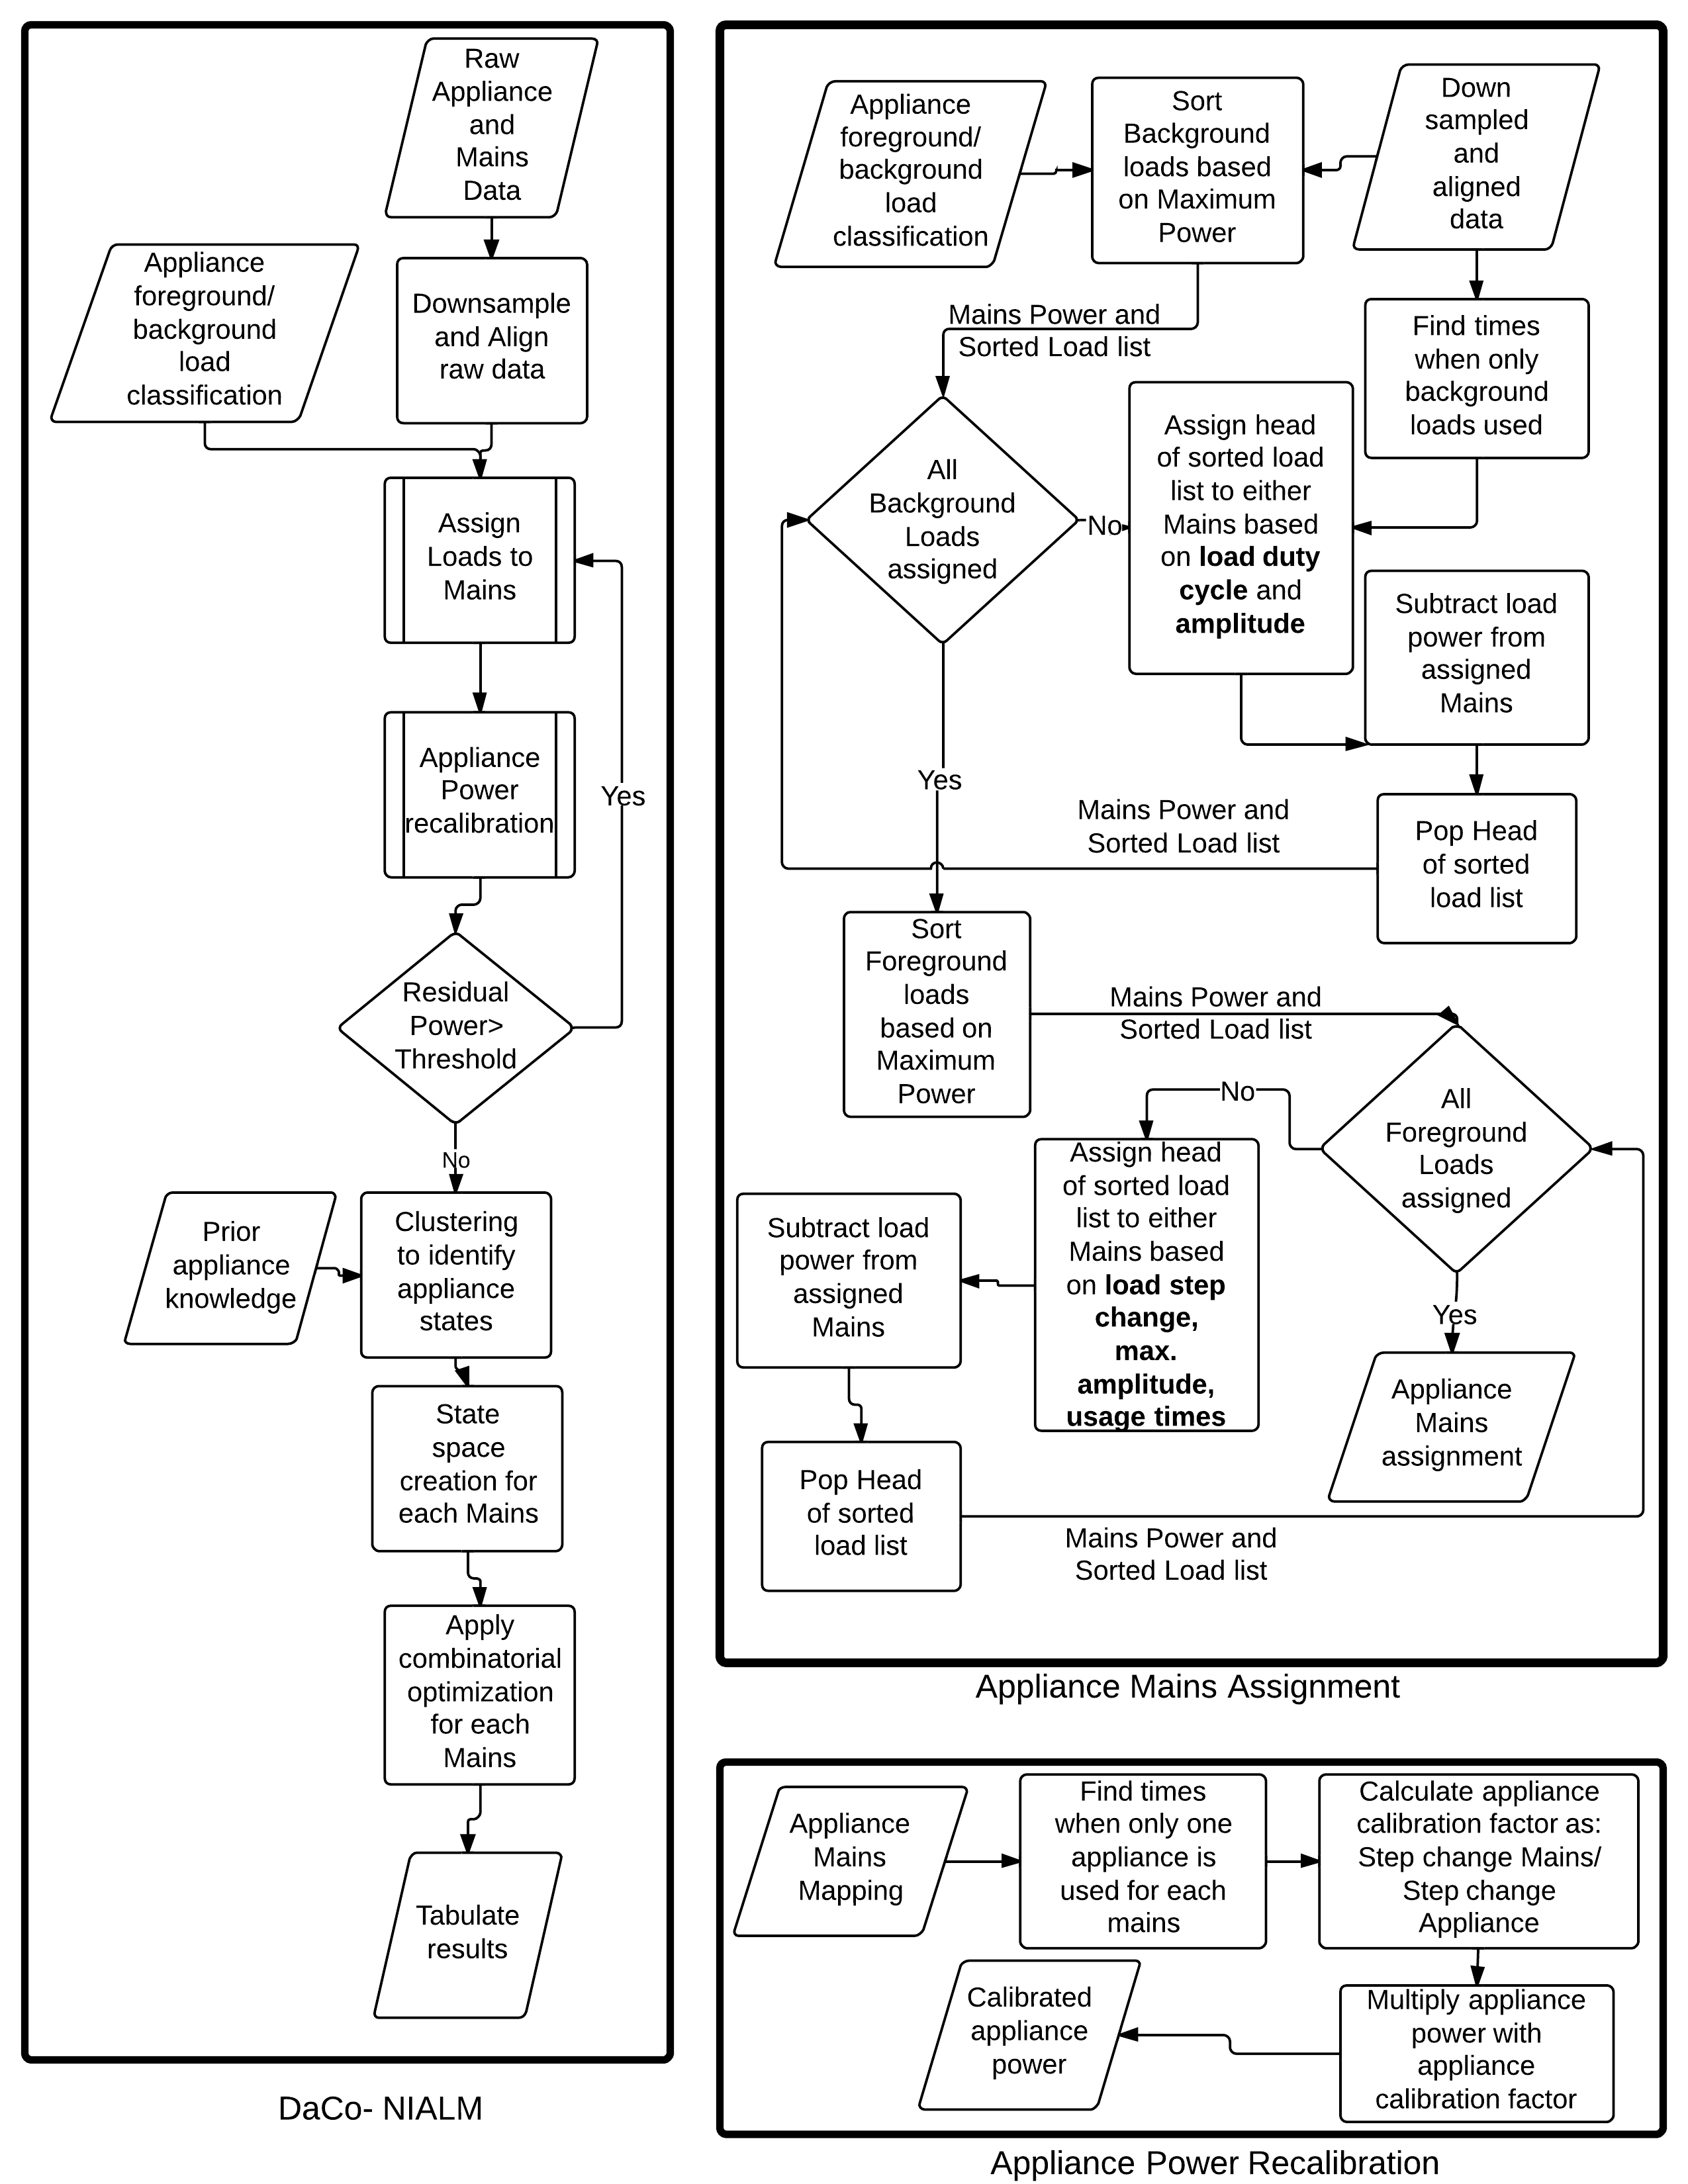
\includegraphics[scale=0.1]{./figures/algo_3.png}
%\caption{Divide and Conquer NIALM}
%   \label{fig:algorithm}
%\end{figure}
In this section we explain the various steps involved in DaCo-NIALM which is shown in \figref{fig:algorithm} or \algoref{algo:main}.

\textbf{Downsample and align raw data}: While performing Combinatorial Optimization it is desired that transients and fluctuations in the power signal are filtered. The transients occur due to the high starting current of the appliance, whereas the fluctuations are a consequence of minor voltage fluctuations and oscillatory nature of loads. \figref{fig:downsample_startup} and \figref{fig:downsample_voltage} show how starting current and voltage fluctuations can be filtered by downsampling. 
%To overcome these we downsampled our data to one minute resolution using mean filter. 
Further realignment amongst the appliance level data and mains level data is needed owing to different frequency of data collection and missing data.
\begin{figure} 
	
    \subfloat[\scriptsize Filtering startup transients]{
    \label{fig:downsample_startup}
    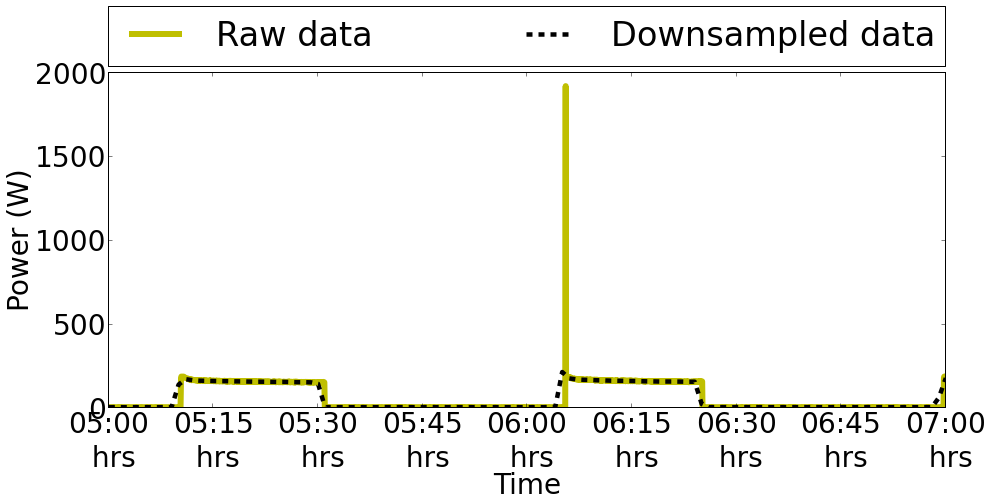
\includegraphics[scale=0.14]{./figures/downsample_1.png}}
    \subfloat[\scriptsize Filtering voltage fluctuations and oscillations]{
        \label{fig:downsample_voltage}
        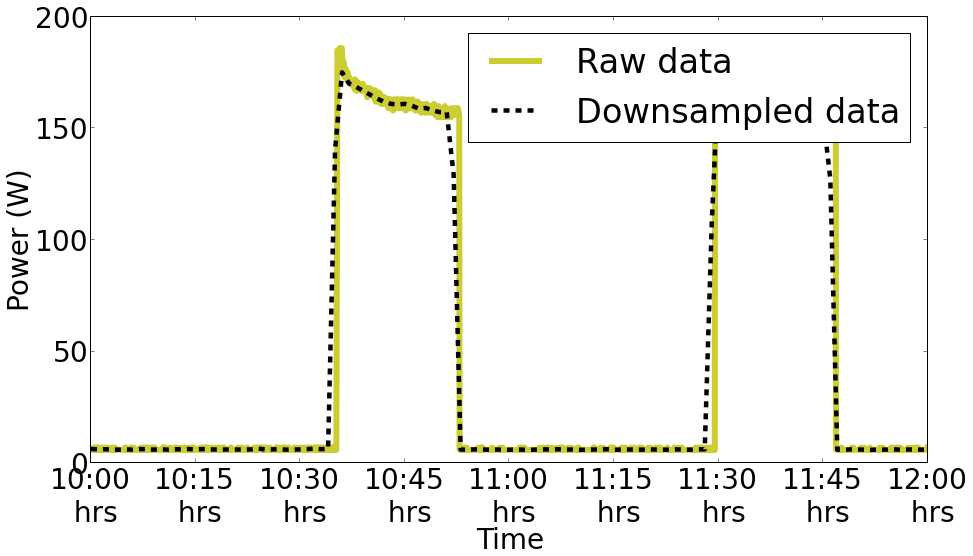
\includegraphics[scale=0.14]{./figures/downsample_2.png}}
  	\caption{Effect of downsampling appliance data}
    \label{fig:downsampling}
\end{figure}

\textbf{Assigning Loads to Mains}:
This step aims to identify the mapping between appliances and mains. Based on domain expertise we label the appliances in a home into background (loads which run independently throughout the day without user interference) such as refrigerator, and foreground (loads which are highly correlated with human usage) such as stove. Background loads are easier to detect since they are On even during periods of low human activity. Also loads with higher mean power consumption are easier to identify and thus we sort background loads based on power in descending order. For all such background loads we see if the mean power of the appliance is greater than mean power of any mains for all time instances. If so, we can safely assign the appliance to the other mains. If this step is unable to provide conclusive evidence we look at the periodicity associated with such background loads during periods of low or no human activity (such as night time). \figref{fig:assignment_1} shows how based on refrigerator duty cycle it is mapped to Mains 2. On similar lines assignment of foreground loads can be done.
\begin{figure} 
	
    \subfloat[\scriptsize Assigning refrigerator to Mains 2 since refrigerator power $>$ Mains 1 power and on basis of duty cycle]{
    \label{fig:assignment_1}
    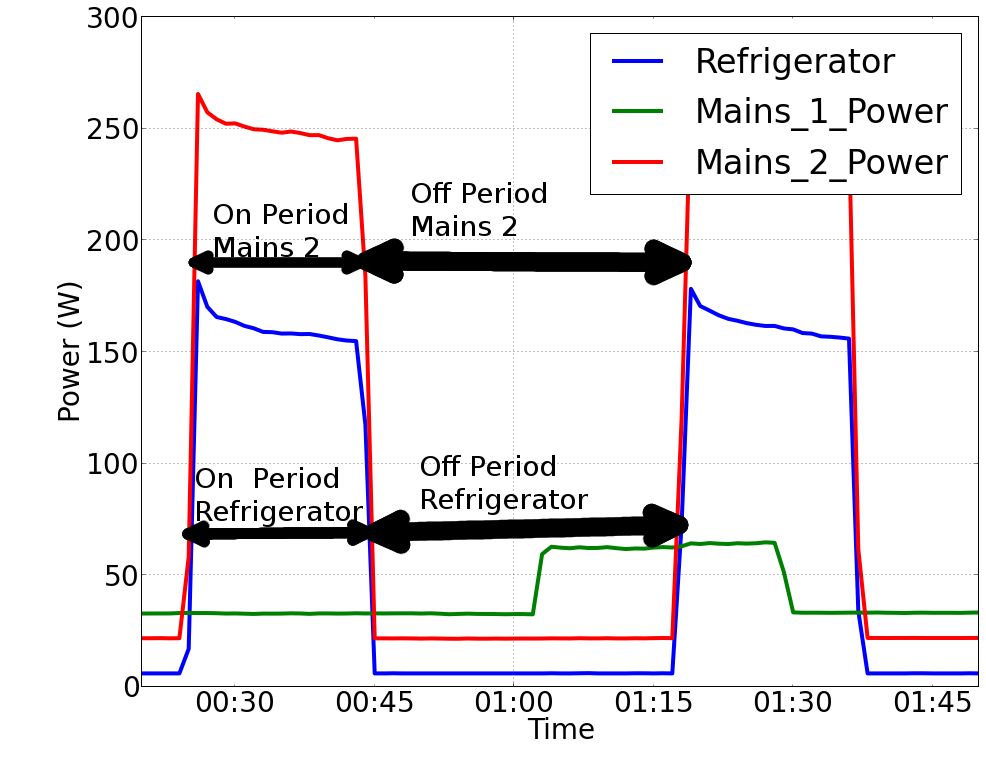
\includegraphics[scale=0.132]{./figures/ref_assign.png}}
    \subfloat[\scriptsize Calibrating Refrigerator Power consumption]{
        \label{fig:assignment_2}
        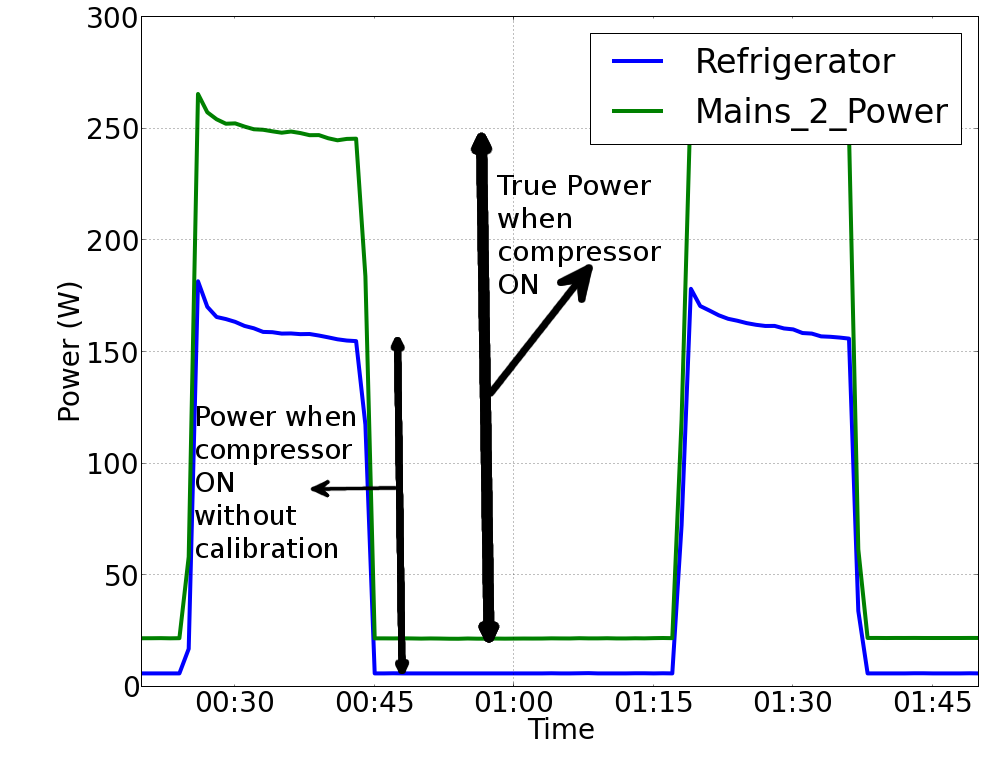
\includegraphics[scale=0.132]{./figures/ref_calibrate.png}}
  	\caption{Calibrating and assigning refrigerator to Mains 2 }
    \label{fig:assignment}
\end{figure}

\textbf{Appliance Power Calibration}: 
Power measured by appliance level meters may need calibration due to the following reasons:
\begin{itemize}
\item Difference in measurement of different measurement instrument (diagram showing CC, ZWave, etc)
\item Fluctuation in voltage cause power to fluctuate as well
\item Missing meta data, whether real or apparent power is being measured at appliance level

\end{itemize}Since different hardware is used for measuring appliance and mains data there may be a need to calibrate the two. Since mains data is usually collected using better precision hardware, we keep mains data as a reference and calibrate appliance data against it. In practice we found appliance level monitors to usually provide only real power whereas the mains monitors can provide much more like reactive and active power. Like the previous step, time instances when an appliance in a particular mains is single used are identified. The ratio of mains and appliance power step changes occurring this window serve as the calibration factor for that appliance. Further each appliance power is corrected with the corresponding calibration factor.

\textbf{Clustering to identify appliance states}:
\begin{enumerate}
\item Step changes occurring in Mains vs Appliances
\item Isolating single appliance usage
We use \cite{kmeansplusplus} to run our clustering
\end{enumerate}
Appliance states identification using clustering (Possibly talk about unbalanced data, but leave it for future work)
State space creation
Applying CO for different mains
Find energy distribution by appliance and assign weights (To be used in results)




\begin{algorithm}
\DontPrintSemicolon % Some LaTeX compilers require you to use \dontprintsemicolon instead 
\KwIn{$x,\theta^n,\theta^{M_1},\theta^{M_2},B,F,v$	}
\KwOut{$y^n,\mu_k^n, Calibrated\: \theta^n$}
\textbf{Align and Downsample}\;
\For {$n \in {1,N}$}
	{
	$\theta^n \gets Downsample(\theta^n,mean,1\: minute)$\;
	}
$\theta^1,..\theta^n,\theta^{M_1},\theta^{M_2} \gets Align([\theta^1,..\theta^n,\theta^{M_1},\theta^{M_2}],forward\: fill)$\;

$s \gets Sort([\theta^1,..\theta^n],peak\: power)$\;

\For{$Appliance\: n \in s$}
	{
	\textbf{Appliance to Mains mapping}\;
	\If {$\theta^n > \theta^{M_1}\: for\: any\: t \in {1,T}$} 
		{ $Mapping[n]=2$\;		
		}  
	\ElseIf {$\theta^n > \theta^{M_2}\: for\: any\: t \in {1,T}$}
		{ $Mapping[n]=1$\;
		}
	\ElseIf {$n \in B$}
		{
		$t \gets Contiguous\_Below\_Mean (\theta^{M_1}, 2\: hours)$\;
		}
	\ElseIf {$n \in F$}
		{
		$t \gets Greater\_Than(\theta^n,100)$
		}
	\Else{
		\If {$Step\_Changes(\theta^n,15,t).Times \subset Step\_Changes(\theta^{M_1},15,t).Times \& 
		Step\_Changes(\theta^n,15,t).Magnitude\/
		Step\_Changes(\theta^{M_1},15,t).Magnitude $}
			{ 
			$Mapping[n]=1$\;
			}
		\Else{
			$Mapping[n]=2$\;	
			}	
		}
	\textbf{Calibration} \;
	$\theta^n \gets \theta^n * Step\_Changes(\theta^n,15,t).Magnitude \/
			Step\_Changes(\theta^{M_{Mapping[n]}},15,t).Magnitude $ \;
	$\theta^n \gets Normalize(\theta^n,v)$\; 
	
	$\theta^{M_{Mapping[n]}} \gets \theta^{M_{Mapping[n]}} - \theta^n $ \;
	
	\textbf{Clustering}\;
	$\mu_k^n \gets Cluster(\theta^n,K,kmeans++) \: for\: k \in {1,K} $\;

	
	}
Solve combinatorial optimization using equation...

\Return{$y^n$}\;
\caption{INDiC}
\label{algo:main}
\end{algorithm}
\subsection{Load assignment}
Draws inspiration from work by Parson et. al \cite{parson2012_aaai}. From prior knowledge we divide the loads into two different categories: Periodic such as refrigerator and non periodic such as Television.

\section{Evaluation}
\subsection{About Dataset}

We use Reference Energy Disaggregation Data Set (REDD) \cite{redd} for validating our algorithms. This dataset contains power and voltage data for mains (2 phases) as well as appliances from 6 homes in Boston area collected in the summer of 2011. The data is made available as raw, high frequency (sampled at 15 KHz) and low frequency (Mains at 1 Hz, appliances at ~0.3 Hz). Considering the practical implications of residential smart meter installation, we believe that low frequency data represents the most realistic scenario and thus we use this data for analysis. 

%\figref{fig:breakdown} shows 6 hourly breakdown of energy consumption across the different mains in Home 2 .


%\begin{figure} 
%	
%    \subfloat[\scriptsize Mains 1]{
%    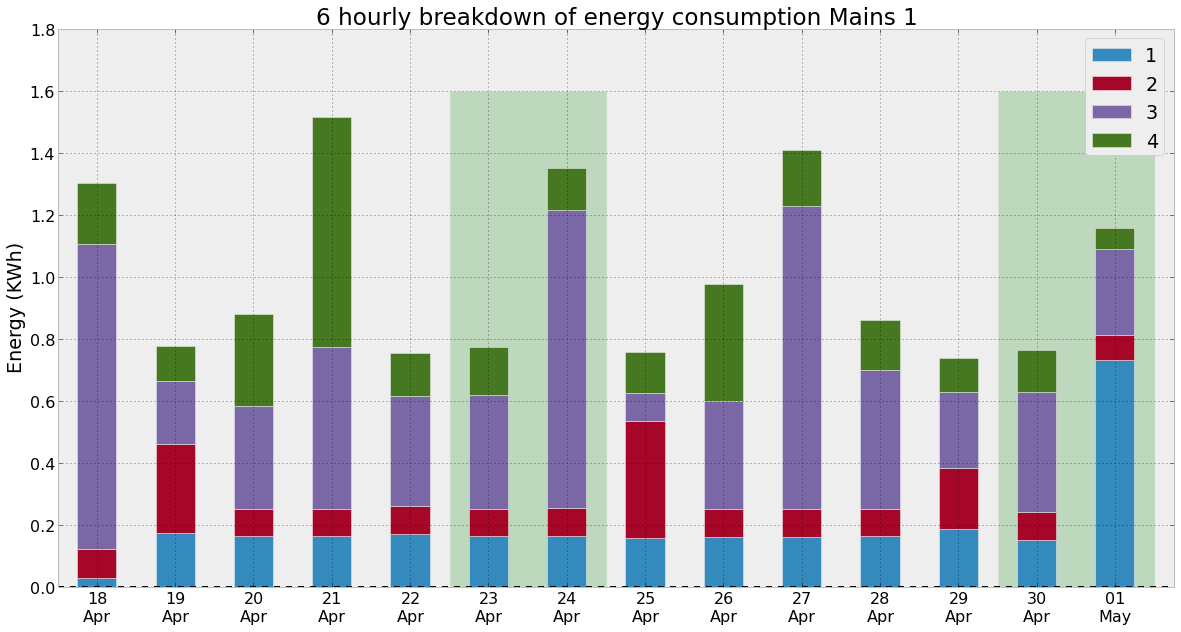
\includegraphics[scale=0.1]{./figures/mains_1_6hr.png}}
%    \subfloat[\scriptsize Mains 2]{
%        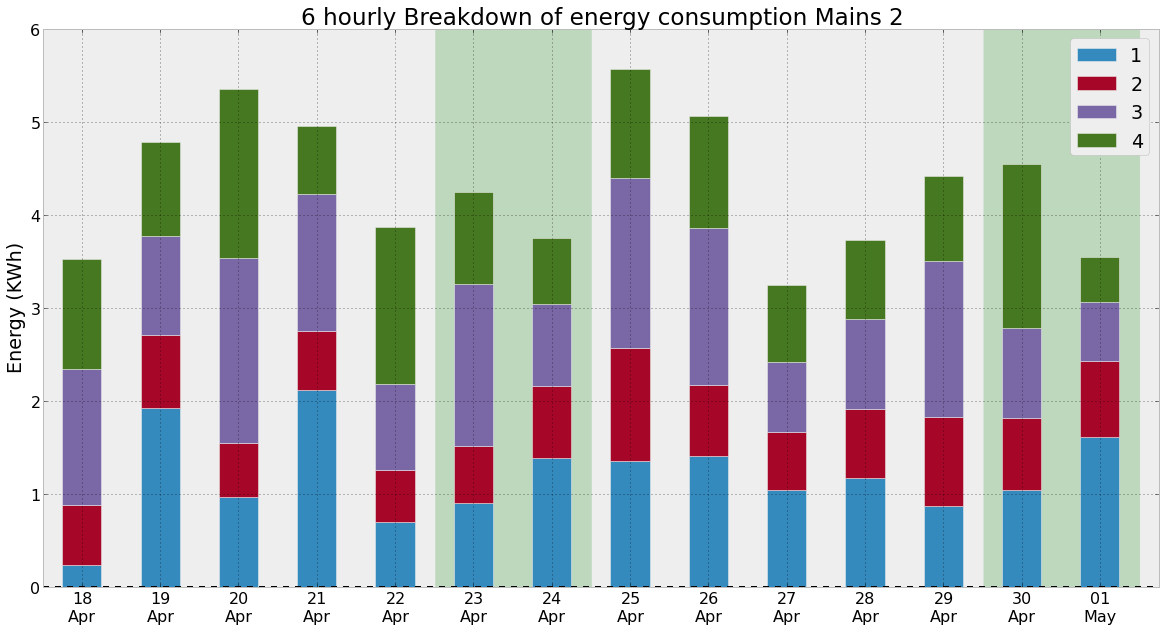
\includegraphics[scale=0.1]{./figures/mains_2_6hr.png}}
%  	\caption{6 hourly energy usage breakdown Home 2}
%    \label{fig:breakdown}
%\end{figure}
%
\subsection{Evaluation Metric}

Commonly used metrics such as accuracy, sensitivity and specificity can be misleading when applied to NIALM. It can be seen from \figref{fig:confusion} that since stove is mostly in state 0 (Off), accuracy will be largely decided by accuracy for this state. This does not tell how badly the prediction is misclassifying state 1 (On). 
%Armel et. al \cite{survey1} discuss the lack of a common metric while comparing NIALM approaches.
Thus, we use the following metrics which have been used in the past work \cite{parson2012_aaai,redd}:
\begin{itemize}
\item \textbf{Mean Normalized Error (MNE \%)}: Normalized error in the energy assigned to an appliance $n$ over time period $T$, given by 
$$ MNE(n)=\frac{|\sum\limits_{t=1}^{T}\theta_t^n- \sum\limits_{t=1}^{T}y_t^n|}{\sum\limits_{t=1}^{T}\theta_t^n} $$


\item \textbf{RMS Error (RE Watts)}: RMS error in power assignment to an appliance $n$ per time slice given by
$$RE(n)=\sqrt{\frac{1}{T}\sum\limits_{t=1}^{T}(\theta_t^n-y_t^n)^2}$$

\end{itemize} 
Since both these quantities represent error, the lesser they are the better is the prediction.
\begin{figure}
\centering 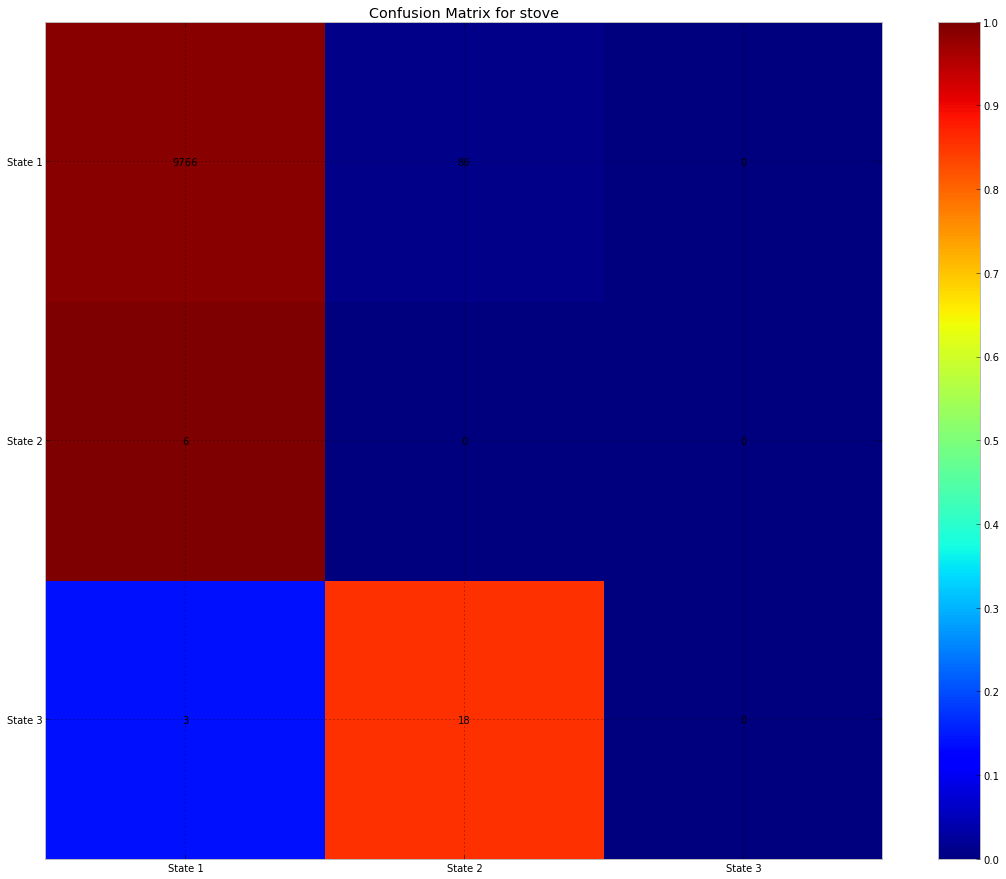
\includegraphics[scale=0.2]{./figures/confusion_stove.png}
\caption{Confusion Matrix showing predicted state accuracy for Stove}
   \label{fig:confusion}
\end{figure}



\subsection{Empirical Analysis}
We performed empirical analysis on REDD dataset Home 2, which consists of 11 channels (including 2 mains and 9 appliances). We believe that the same analysis can be easily repeated across multiple homes. We aligned the data and downsampled it to one minute using mean filter. Since we had two weeks of clean data, we used the first week as the train set and the second week as the test set. We used INDiC algorithm described earlier to assign loads to different mains and calibrate appliance data. \tabref{tab:calibration_factors} shows the assignment of loads to different mains. Further this table also shows the learnt power states of these appliance via k-means++ clustering (which for several reasons is considered better than k-means) \cite{kmeansplusplus}. Refrigerator and lighting showed significant difference in power states post calibration. Based on prior experience and appliance circuity, we believe that since only these two appliances needed calibration, it may be a case that the appliance level monitor measured real power instead of apparent power. These loads constitute a major chunk of Mains 2 power. \figref{fig:calibration} shows the reduction in unassigned power due to calibrating these two appliances. Two loads - washer dryer and disposal did not have significant usage and we chose not to consider them in the analysis. 

To show the significance of load division and calibration, we applied Combinatorial optimization on the test set, considering 4 possible cases:  i) no calibration, no load division; ii) no calibration, load division; iii) calibration, no load division; iv) calibration, load division. These results are presented in \tabref{tab:results}. For the overall dataset, it can be seen that MNE reduces from 187\% to 39\%, RE reduces from 478 W to 168 W, after applying INDiC. All appliances show reduction in MNE and RE after applying INDiC. However, there is significant improvement in correctly predicting refrigerator and lighting. \figref{fig:confusion_ref} shows the confusion matrix for refrigerator prediction pre and post applying INDiC. It can be seen that after applying INDiC there is a vast improvement in predicting refrigerator's state 0 and 1.

We had used Combinatorial Optimization which is the simplest NIALM technique to show the improvements which can be made by load division and appliance calibration. We believe that using state of the art NIALM algorithms will improve the results by leaps and bounds.

%\item Overall results in \tabref{tab:results}, first column NILM without dividing into mains and without recalibration, last column with DiCaCo NIALM. Vast reduction in R.E. and M.N.E , especially for most appliance contributing most like refrigerator and lighting	
%\item Confusion matrix showing a large improvement in refrigerator recognition in \figref{fig:confusion_ref}
%\end{itemize}

\begin{figure} 
	
    \subfloat[\scriptsize Without applying calibration]{
    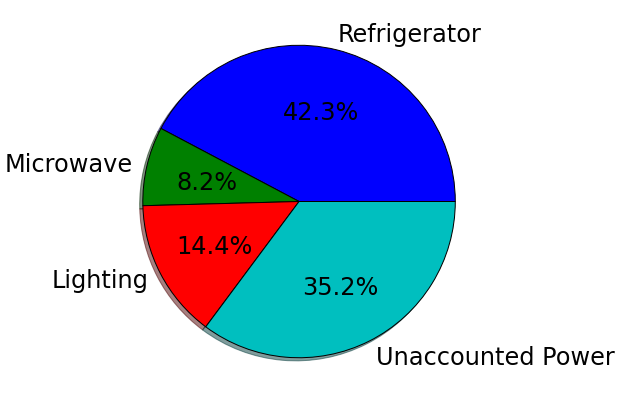
\includegraphics[scale=0.2]{./figures/breakdown_before_calibration.png}}
    \subfloat[\scriptsize After applying calibration]{
        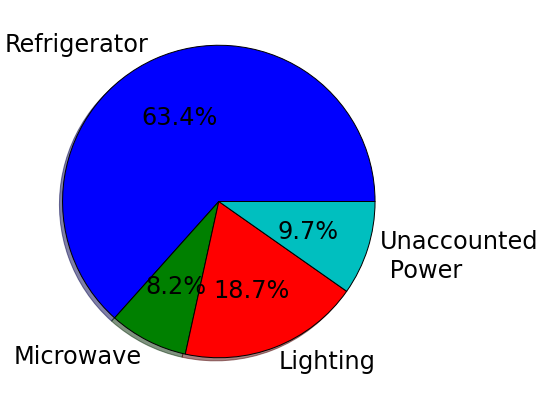
\includegraphics[scale=0.2]{./figures/breakdown_after_calibration.png}}
  	\caption{Mains 2 Break down by load}
    \label{fig:calibration}
\end{figure}
\begin{figure} 
	
    \subfloat[\scriptsize Without applying DiCaCo]{
    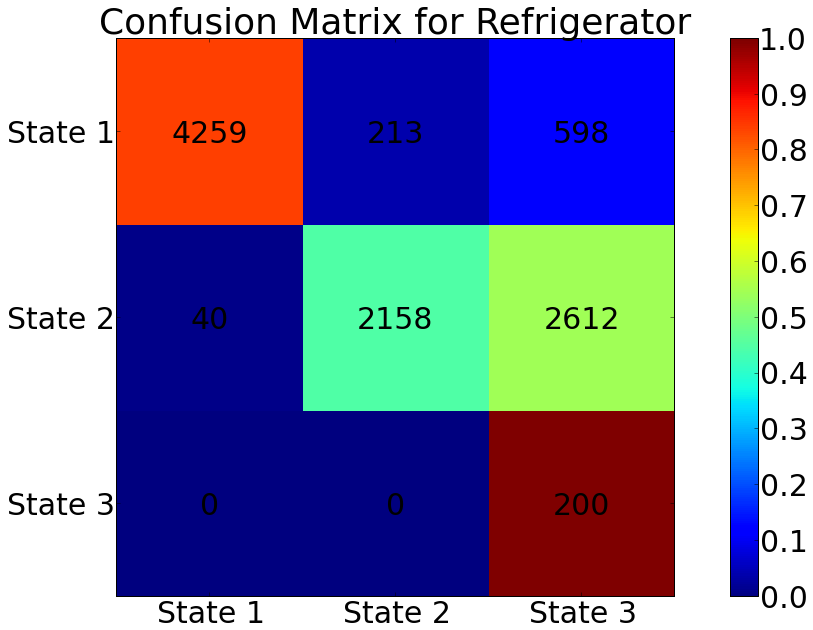
\includegraphics[scale=0.15]{./figures/confusion_before_dicaco.png}}
    \subfloat[\scriptsize After applying DiCaCo]{
        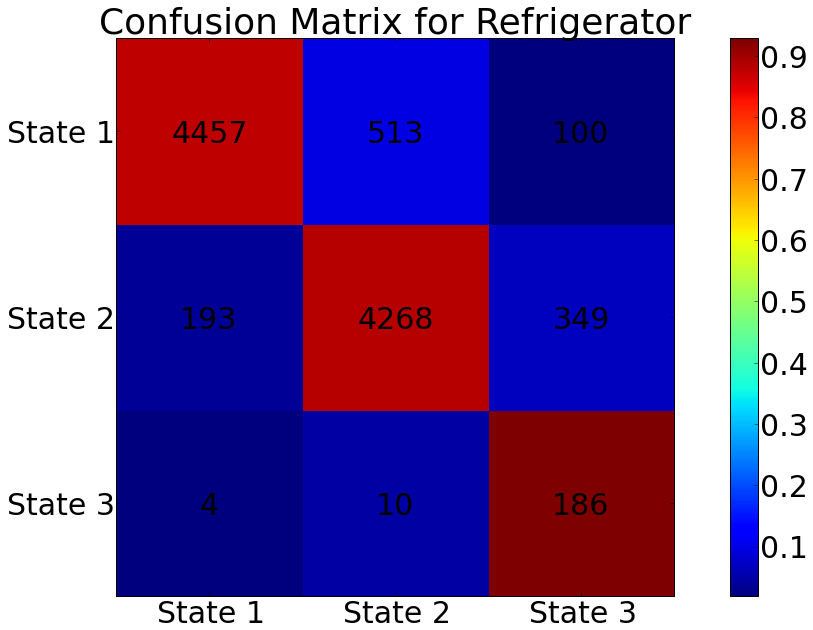
\includegraphics[scale=0.15]{./figures/confusion_after_dicaco.png}}
  	\caption{Confusion Matrix for refrigerator disaggregation}
    \label{fig:confusion_ref}
\end{figure}

%\item Table on Calibration factors
\begin{table}
%%% increase table row spacing, adjust to taste
%%\renewcommand{\arraystretch}{1.3}
%% if using array.sty, it might be a good idea to tweak the value of
%% \extrarowheight as needed to properly center the text within the cells
\caption{Calibration Factors, Mains Assignment and States}
\label{tab:calibration_factors}
%\centering
%%% Some packages, such as MDW tools, offer better commands for making tables
%%% than the plain LaTeX2e tabular which is used here.
\begin{tabular}{|c|c|c|c|}
\hline
Appliance & Mains & States Power (W)& States Power (W)\\
\hline
&&Pre calibration&Post calibration\\
\hline
Refrigerator & 2& 7,162,423 & 9,210,423\footnote{Could not be calibrated}\\
Microwave &2& 10,832,1730& 10,832,1730\\
Lighting & 2& 9,96,156&10,110,178\\
Dishwasher & 1& 0,256, 1195 & 0,256, 1195\\
Stove& 1 & 0,374& 0,374\\
Kitchen & 1& 5,727&5,727\\
Kitchen 2&1 & 1,204,1032&1,204,1032 \\
%
%
\hline
%
\end{tabular}
\end{table}

\begin{table}
\caption{Mean Normalized Error and RMS error with and without DiCaCo NIALM}
\label{tab:results}
\begin{tabular}{|p{30pt}|p{12pt}|p{14pt}|p{12pt}|p{14pt}|p{12pt}|p{14pt}|p{12pt}|p{14pt}|}
\hline
&\multicolumn{4}{|c|}{Without}&\multicolumn{4}{|c|}{With}\\
&\multicolumn{4}{|c|}{Recalibration}&\multicolumn{4}{|c|}{Recalibration}\\
\hline
&\multicolumn{2}{|c|}{Without Load}&\multicolumn{2}{|c|}{With Load}&\multicolumn{2}{|c|}{Without Load}&\multicolumn{2}{|c|}{With Load}\\
&\multicolumn{2}{|c|}{Division}&\multicolumn{2}{|c|}{Division}&\multicolumn{2}{|c|}{Division}&\multicolumn{2}{|c|}{Division}\\
\hline

Appliance &R.E.&M.N.E.& R.E.&M.N.E.&R.E.&M.N.E.&R.E.& M.N.E.\\
&Watts&\%&Watts&\%&Watts&\%&Watts&\%\\
\hline
Refrigerator & 136 &109 & 71 & 32 & 130 &95  &59 &21\\
Microwave    & 102 &98  & 97 & 110& 104 &97  &96 &109\\
Lighting     & 51  &164 & 48 & 195& 44  &83  &38 &60\\
Dishwasher   & 406 &2947& 63 & 100& 377 &2517&63 &100\\
Stove        & 77  &1191& 36 & 281& 75  &1118&36 &281\\
Kitchen      & 64  &182 & 58 & 168& 69  &196 &58 &168\\
Kitchen 2    & 95  &267 & 91 & 117& 92  &230 &91 &117\\
\hline
Overall      &478  &187 &161 &  58& 450 &157 &168&39\\

\hline

\end{tabular}
\end{table}





\section{Conclusion}
The conclusion goes here.
We also provide mains load assignment of all 6 homes from REDD to further the research in this direction.

\section{Future Work}
\begin{itemize}

\item Applying model on noisy datasets
\item 2 D CO (when Real and Reactive Power are known)
\item Factoring in Time of Day etc.
\item Factoring in Appliance Correlation
\item Factor in switch continuity, essentially leads to Factorial HMM
\item Distributed NILM
\item Adaptive Learning
\end{itemize}

\section*{Acknowledgment}
The authors would like to thank TCS Research and Development for supporting the first author through PhD. fellowship. We would also like to thank NSF- DEITy for funding the project.
\bibliographystyle{IEEEtran}
\bibliography{IEEEabrv,references}

\end{document}


